\chapter{Introduction}

\section{Background}

%paragraph 1 Forecasting models play an important role in water quality control in DTPs and WWTPs.
%paragraph 2 Water reclamation-why is it a good choice for solving urban water scarcity
%paragraph 3 Decision-making processing-how does this help water reclamation
%paragraph 4 Deep learning model to replace fuzzy supervisor and machine learning models-the need of using it
AI technologies have been successfully applied to different DWT processes, such as the prediction of the coagulant 
dosage, discrimination of the DBP formation potential, advanced control of membrane fouling, membrane preparation 
and optimization, and water quality prediction. \cite{liRecentAdvancesArtificial2021}

%%%% Paragraph 1
Forecasting models play an important roles in water quality control in drinking water treatment plants (DTPs) 
and wastewater treatment plants (WWTPs). The need of using forecasting models are becuase the unpredictable 
nature of water quality, and the treatment operations are subjected to the change of water quality to prodcue
effluent complied the government regulation \cite{chenAssessingWastewaterReclamation2003}

%%%% Paragraph 2
Forecasting models can also be called time series model becuase the data is consisted of the values and the 
time (need to be further revised). For the well-know time series models are for example, RNN, ... These are 
used to replace the theory-based models, for example Activated Sludege Model (ASM). The difference between 
these two models are, machine learning based models require to learn from historic data, while the thoery-based
models only need to enter the basic operational parameters (e.g., influent flow, tempearture, and pH, etc).

%%%% Paragraph 3
Despite the promising usage and performance of machine learning models, the collection of the data became
the most difficult tasks. Many small scale or old treatment plants do not have the capital or the available
environment for the set-ups of the online sensors to collect data.
Although these are the major issues, it's still possible to train a forecasting model with one input, which 
is also called a self-prediction model. Although the accuracy or stability compared to multi-input models, 
the forecasted results can be used at some cases. To increase the model performance, there are several ways.
Paper included weather data, or perform data-preprocessing methods to improve the model performance.

%%%% Paragraph 4
These solutions (data preprocessing, feature engineering) are not well discussed in this field, also the 
potential of using univariate models are under estimated.

Keeping an effective disinfectant residual concentration in reclaimed water is still a challenge, due to its high levels of ammonia and organic matter when compared with those in drinking water. \citep{costaIdentificationModellingChlorine2021}


%\begin{figure}[!t]
%   \centering
%   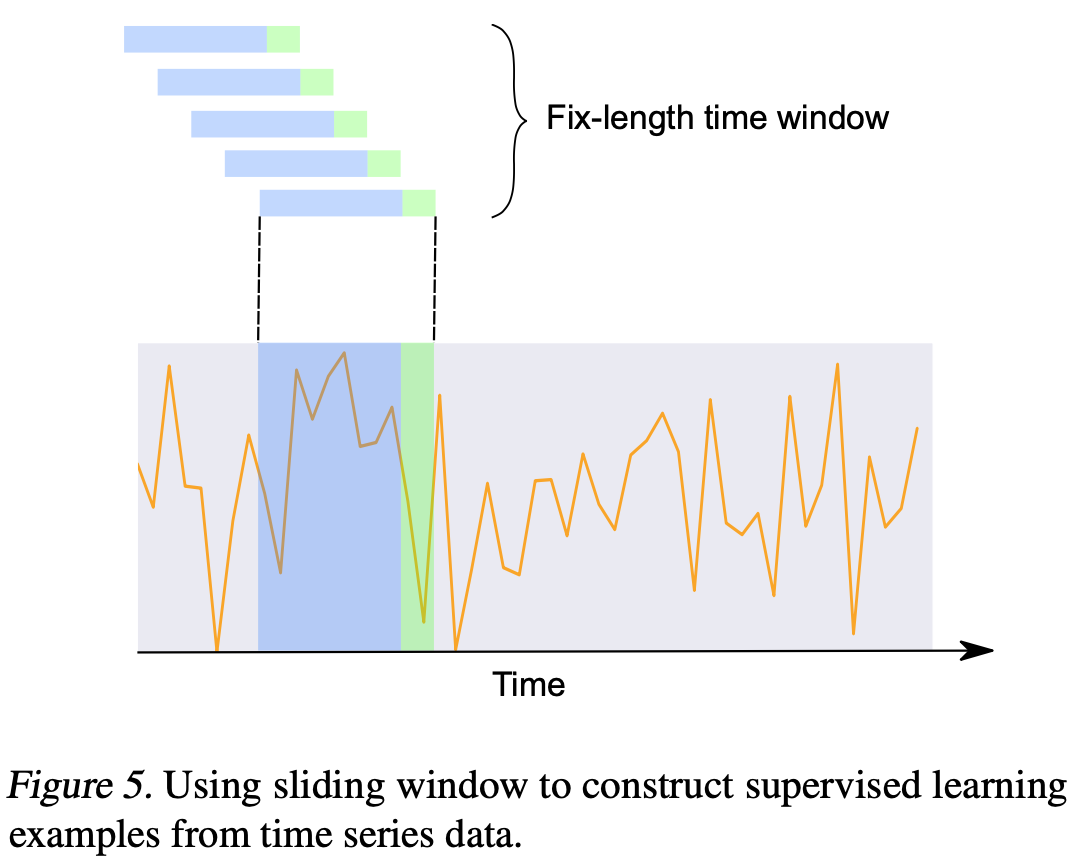
\includegraphics[width=0.75\columnwidth]{imgs/fix-length-time-window.png}
%   \caption{The network structure for the actor-evaluation estimation. It is a combination of convolutional networks for feature extraction and fullyconnected layers for policy learning. They have been separately proven to be effective in our previous works.}
%   \label{fig:ob_network_structure}
%\end{figure}

\section{Objectives}
\noindent
The specific objectives of this thesis work are:\\
%should be investigate the effluent water quality in SWHEPP?
(1) To build baseline univariate forecasting models using machine learning and deep learning models.\\
(2) To develop data preprocessing methods for enhancing model forecasting performance.\\
(3) To extract features and hidden relations of water parameters in MBR effluent by analyzing the wastewater collected upstream of the WWTPs.\\
(4) To develop methods for improving performance of forecasting models using the hidden features and relations of the water parameters.

\section{Organization of the thesis}